% === Begin Label Data ===
% ID: 486
% 难度星级: 
% 标签: 
% 备注: 
% 组卷引用次数: 0
% === End  Label Data ===

\begin{problem}{2020}{G}{新高考I卷}{10}{三角函数}
下图是函数 $ y=\sin(\omega x+\varphi) $ 的部分图象，则 $ \sin(\omega x+\varphi)= $
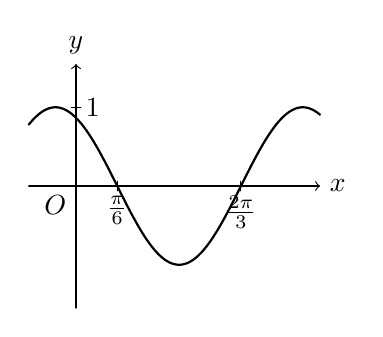
\begin{tikzpicture}[line cap=round,line join=round,scale=1]
\def\xmin{-0.6}
\def\xmax{3.1}
\def\ymin{-1.55}
\def\ymax{1.55}

\draw[->] (\xmin,0) -- (\xmax,0) node[right] {$x$};
\draw[->] (0,\ymin) -- (0,\ymax) node[above] {$y$};
\node[below left] at (0,0) {$O$};

\draw (-0.06,1) -- (0.06,1);
\node[right] at (0,1) {$1$};

\draw ({pi/6},-0.06) -- ({pi/6},0.06);
\node[below] at ({pi/6},0) {$\frac{\pi}{6}$};

\draw ({2*pi/3},-0.06) -- ({2*pi/3},0.06);
\node[below] at ({2*pi/3},0) {$\frac{2\pi}{3}$};

\draw[thick,domain=\xmin:\xmax,samples=200]
  plot (\x,{sin((pi/3-2*\x) r)});
\end{tikzpicture}
\begin{choices}
\choice{{$\sin\left(x+\dfrac{\pi}{3}\right)$}}
\choice{{$\sin\left(\dfrac{\pi}{3}-2x\right)$}}
\choice{{$\cos\left(2x+\dfrac{\pi}{6}\right)$}}
\choice{{$\cos\left(\dfrac{5\pi}{6}-2x\right)$}}
\end{choices}
\end{problem}

\begin{answer}

\end{answer}

\begin{solutions}

\end{solutions}